%% =====================================================================
%% Aggregate accuracy conceals an acquisition-level failure in a public
%% radar target recognition benchmark.
%%
%% SINGLE-COLUMN version, for a venue allowing up to 12 pages. The
%% two-column 6-page conference version is paper_main.tex; the two share
%% no text, so a number corrected in one must be corrected in the other.
%% check_expected.py verifies both against the released reports, which is
%% what keeps them from drifting apart silently.
%%
%% RETARGETING. The body uses only standard sectioning, booktabs,
%% graphicx and tikz, so moving to a publisher class is a preamble edit.
%%   IEEEtran, one column : \documentclass[journal,onecolumn,11pt]{IEEEtran}
%%                          and restore \IEEEauthorblockN in the author block
%%   Elsevier             : \documentclass[preprint,12pt]{elsarticle}
%%                          \begin{frontmatter} around title/author/abstract
%%   MDPI                 : \documentclass[journal,article,submit]{Definitions/mdpi}
%%   Springer Nature      : \documentclass[pdflatex,sn-basic]{sn-jnl}
%% In each case delete the geometry line below and let the class set the
%% page. Nothing in the body needs to change. Current setting is 11pt on
%% A4 with 2.5cm margins, which is looser than any of the four classes
%% above, so the page count below is an upper bound on all of them.
%%
%% FIGURES expected in figures/ alongside this file:
%%   recall_by_acquisition.png   doppler_by_acquisition.png
%%   session_13-48_compact.png
%% TABLES generated by tools/make_tables.py into tables/:
%%   acquisitions.tex            compression.tex
%% Regenerate with:  python tools/make_tables.py
%%
%% Every number here comes from a measured run in reports/ and is checked
%% by check_expected.py. No placeholders remain.
%% =====================================================================
\documentclass[10pt,a4paper]{article}

\usepackage[T1]{fontenc}
\usepackage[utf8]{inputenc}
\usepackage[margin=2.4cm]{geometry}
\usepackage{times}
\usepackage{amsmath,amssymb}
\usepackage{graphicx}
\graphicspath{{figures/}}
\usepackage{booktabs}
\usepackage{url}
\usepackage{tikz}
\usetikzlibrary{arrows.meta,positioning}
\usepackage[hidelinks]{hyperref}
\usepackage{caption}
\captionsetup{font=small,labelfont=bf}

\setlength{\parskip}{1pt}
\setlength{\textfloatsep}{10pt plus 2pt minus 2pt}
\setlength{\intextsep}{10pt plus 2pt minus 2pt}

%% Heading spacing. The class defaults put roughly a line and a half of air
%% around each of the thirty-odd headings here, which costs close to a page
%% in total. These values keep headings clearly separated and reclaim it.
\usepackage{titlesec}
\titlespacing*{\section}{0pt}{8pt plus 2pt minus 2pt}{4pt}
\titlespacing*{\subsection}{0pt}{6pt plus 1pt minus 1pt}{2pt}
\titleformat*{\section}{\large\bfseries}
\titleformat*{\subsection}{\normalsize\bfseries}
\setlength{\abovecaptionskip}{4pt}
\setlength{\belowcaptionskip}{0pt}

%% Let floats share a page with more text. The defaults reserve so much of
%% each float page for the float that three pages here were left a quarter
%% empty, which costs a whole page over the paper and buys nothing.
\renewcommand{\topfraction}{0.92}
\renewcommand{\bottomfraction}{0.85}
\renewcommand{\textfraction}{0.07}
\renewcommand{\floatpagefraction}{0.8}
\newcommand{\s}[1]{\texttt{#1}}            % an acquisition name
\newcommand{\tgt}{\s{13-48}}               % the acquisition this paper is about

\title{\bfseries Aggregate Accuracy Conceals an Acquisition-Level Failure\\
in a Public Radar Target Recognition Benchmark}

\author{Ghulam Mustafa \and Ghulam Murtaza \and Ali Nawaz \and Zohaib Ahmad Khan}
\date{College of Aeronautical Engineering,
National University of Sciences and Technology, Islamabad, Pakistan\\[2pt]
\small\texttt{gmustafa.ms19avecae@student.nust.edu.pk}}

\begin{document}
\maketitle

\begin{abstract}
\noindent
Public radar target recognition datasets are commonly evaluated with random train/test partitions over individual range--Doppler frames. Because frames come from continuous recordings, this never asks whether a classifier generalises to an acquisition it has not seen. We report an acquisition-level audit of the Real Doppler RAD-DAR database, reconstructing its structure into 52 grouping units from 80 folders after removing a duplication of the directory tree in the distributed archive. A session-grouped protocol lowers mean accuracy from 0.9335 to 0.9099 and mean drone recall from 0.9358 to 0.8376, differences dominated by one fold rather than spread evenly. The per-acquisition breakdown is the more informative view, and one cross-validation pass yields it free: of twenty-one drone acquisitions, twenty attain out-of-fold recall above 0.90 while one, \tgt, attains 0.249. Excluding that acquisition from training entirely leaves recall on a held-back half at 0.178 over ten seeds; adding the other half raises it to 0.948, with no overlap between conditions on any seed, while the same experiment on the weakest acquisition of each other class recovers only 0.056 and 0.008. Low recall and a large recovery are therefore separate properties. The acquisition is distinguished from all others by Doppler position, at centroid 8.50 against 29.70 to 31.19, and by a within-acquisition spread of 10.64 bins against 0.64 to 2.37. A three-frame approximation to the published baseline's temporal input raises random-split accuracy to 0.9794, within a quarter of a point of the best published figure for a model of this size, and still leaves that acquisition at 0.367; sixteen combinations of input resolution and weight precision, and Doppler shift augmentation at three strengths, also fail on it. A sliding window over a random split places 82.7\,\% of test frames inside some training input, yet removing that overlap entirely costs only 0.0063 in accuracy, which we report because the audit alone would have supported a stronger claim. We present this as a single-acquisition case study of one benchmark and argue that acquisition-level breakdowns should accompany aggregate accuracy on benchmarks assembled from continuous recordings.
\end{abstract}

\noindent\textbf{Keywords:} radar target recognition; evaluation protocol; cross-validation; FMCW radar; drone detection; model compression; negative results

% =====================================================================
\section{Introduction}
\label{sec:intro}

Automatic target recognition from frequency modulated continuous wave (FMCW) radar has been widely addressed with convolutional networks operating on range--Doppler representations. On the Real Doppler RAD-DAR database, the benchmark studied here, published classifiers report accuracies between 98 and 99\,\%~\cite{roldan2020,zhang2025}, and the reported figure is in both cases obtained by partitioning the available frames at random.

That choice deserves scrutiny. The dataset is assembled from continuous recordings, so consecutive frames within one acquisition are strongly correlated, and a random partition places frames from a single acquisition on both sides of the split. The reported accuracy then describes performance on acquisitions the model has already seen, not on a recording absent from training. The question is what that protocol hides, and the answer turns out to be concentrated rather than diffuse: not a uniform overstatement of a few points, but one recording on which the classifier fails outright while the aggregate stays healthy.

Our contributions are: a reproducible preparation procedure that removes a duplication of the directory tree in the archive and recovers acquisition structure from the directory hierarchy, yielding 52 grouping units from 80 folders (Section~\ref{sec:data}); a five-fold comparison of random against session-grouped partitioning in which we do not establish a significant aggregate difference, with the reasons such comparisons are hard to test (Section~\ref{sec:leak}); a per-acquisition breakdown of all 52 units, a controlled exposure experiment associating the one severe failure with absent training coverage rather than intrinsic difficulty, and two controls showing that low recall and a large recovery are separate properties (Section~\ref{sec:regime}); a four-arm design separating temporal information, companion distance and the train/test overlap a sliding window creates, which rules out our single-frame input as the cause (Section~\ref{sec:temporal}); a resolution-by-precision study which does not reproduce on this dataset the disparate-impact-of-compression result established in vision (Section~\ref{sec:compress}); and four mechanisms, each formulated in advance and none supported by the measurements this dataset permits (Section~\ref{sec:mech}).

We report negative results deliberately, and state the scope plainly: both principal observations concern the same acquisition, so the effective sample size at that level is one. This is a case study of one benchmark, not a general result about radar target recognition, and nothing here establishes how common such acquisitions are.

% =====================================================================
\section{Related Work}
\label{sec:related}

The Real Doppler RAD-DAR database was released with a convolutional baseline, DopplerNet, reporting 99.48\,\% accuracy on the three-class problem of vehicles, drones and pedestrians~\cite{roldan2020}. The acquisition hardware is described separately~\cite{quevedo2019}. A recent lightweight architecture reports 98.08\,\% average accuracy on the same data with a model footprint of roughly 400\,kB~\cite{zhang2025}, and provides the per-class confusion matrices we use as an external reference in Section~\ref{sec:model}. Both figures come from random partitions of the frame pool, and Section~\ref{sec:published} examines what each actually measures, since they are defined differently from one another and differently again from the numbers we report.

That correlated samples inflate apparent performance is not a new observation. Grouped partitioning is standard practice in human activity recognition, where subject-disjoint splits are routine, and radar recognition studies have used track-level separation to limit correlation between training and test segments~\cite{buchman2022}. Our contribution is not the idea that grouping matters, but the acquisition-level audit of one widely reused benchmark, which localises a concrete failure regime its aggregate accuracy does not reveal, with a controlled experiment associating that failure with coverage rather than difficulty.

Nor is the difficulty of conditions absent from training a new concern in radar. Recent work addresses single-source domain generalisation for low-slow-small target recognition under changing conditions~\cite{chen2025}, and open-set recognition that rejects classes not present in training~\cite{bai2026}. The acquisition we study is not an unknown class, so open-set rejection is not the remedy: its label is correct and its samples sit nearest the drone centroid by every measure we computed. It is an in-class regime the training distribution does not cover, which is harder to detect because nothing about it looks anomalous at the label level.

Comparing learning procedures across resampled partitions is statistically delicate: commonly used tests have inflated Type~I error on cross-validation scores~\cite{dietterich1998}, and the dependence from overlapping training sets must enter any variance estimate~\cite{nadeau2003}. We take this seriously enough to decline a significance test on our protocol comparison rather than report a $p$ value whose assumptions we cannot defend. Separately, that compression damages some classes or examples more than others is established in vision~\cite{hooker2019,hooker2020,tran2022}; Section~\ref{sec:compress} tests the radar instantiation on this dataset and does not reproduce it, which we report as a non-replication on one benchmark rather than as a refutation.

% =====================================================================
\section{Dataset and Preparation}
\label{sec:data}

\begin{figure}[tb]
\centering
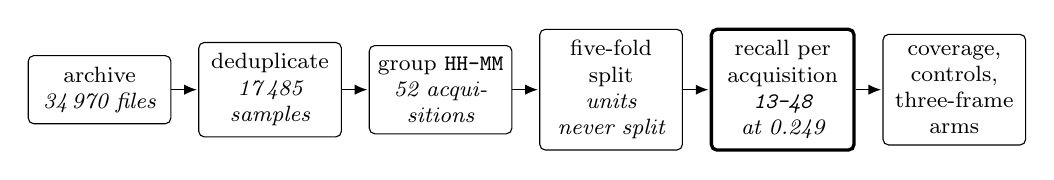
\begin{tikzpicture}[
  bx/.style={draw, rounded corners=2pt, align=center, inner xsep=3pt,
             inner ysep=4pt, text width=0.132\textwidth, font=\footnotesize},
  hl/.style={bx, very thick},
  ar/.style={-{Latex[length=1.6mm,width=1.3mm]}, shorten >=0.5pt}]
\node[bx] (a) {archive\\{\itshape 34\,970 files}};
\node[bx, right=3.4mm of a] (b) {deduplicate\\{\itshape 17\,485 samples}};
\node[bx, right=3.4mm of b] (c) {group \s{HH-MM}\\{\itshape 52 acquisitions}};
\node[bx, right=3.4mm of c] (d) {five-fold split\\{\itshape units never split}};
\node[hl, right=3.4mm of d] (e) {recall per acquisition\\{\itshape \tgt{} at 0.249}};
\node[bx, right=3.4mm of e] (f) {coverage, controls,\\three-frame arms};
\draw[ar] (a) -- (b); \draw[ar] (b) -- (c); \draw[ar] (c) -- (d);
\draw[ar] (d) -- (e); \draw[ar] (e) -- (f);
\end{tikzpicture}
\caption{Preparation and evaluation. The bold step is the one a frame-level
protocol does not produce, and it is free: every unit is held out exactly
once, so one cross-validation pass yields a recall per acquisition, and that
breakdown is what exposes \tgt.}
\label{fig:pipeline}
\end{figure}

\subsection{Acquisition and signal parameters}

The database was collected with an FMCW system at 8.75\,GHz with 500\,MHz of bandwidth, using one transmitting and eight receiving antennas forming a 64-element array~\cite{roldan2020,quevedo2019}. The published parameters give a range resolution of 0.878\,m, a maximum unambiguous range of 3.598\,km and a Doppler resolution of 0.34\,km/h with 512 integrated ramps. We quote these rather than recomputing them: a naive calculation from bandwidth alone gives a range resolution roughly three times finer than the system achieves.

Samples are supplied as $11 \times 61$ matrices obtained by applying a constant false alarm rate detector to the full range--Doppler matrix and cropping around each detection. The retained Doppler window spans approximately 21\,km/h, considerably narrower than the extent associated with rotor blade returns from a small rotorcraft, so the crops do not retain what is needed to analyse blade-flash structure. That is one reason several mechanisms in Section~\ref{sec:mech} are untestable here rather than tested and rejected, and it is not a claim that the crops hold no micro-Doppler information at all.

\subsection{Duplication in the distributed archive}

The distributed archive carries the directory tree twice, once beneath a \s{data/} prefix and once at the archive root, so a naive load doubles every sample and halves the effective size of any held-out set. Hashing each folder identifies the copies; the digest samples twelve files spread across a folder and the first 64\,kB of each, which is an engineering check for identical copies rather than an exhaustive byte-level comparison. After deduplication the totals are 5720 vehicle, 5065 drone and 6700 pedestrian samples, 17\,485 in all, matching the published figure exactly~\cite{zhang2025}, which is the evidence that the deduplication is correct rather than merely plausible. A second pass drops any folder whose name duplicates another of the same class but holds fewer files, guarding against a truncated copy left by an interrupted extraction.

\subsection{Recovering acquisition structure}
\label{sec:grouping}

Acquisition structure is encoded in the directory hierarchy rather than in file names, which are running indices. Folders are named by acquisition time, with suffixes distinguishing variants recorded in the same session, for example \s{15-55}, \s{15-55a}, \s{15-55m} and \s{15-55p}. We group by the leading \s{HH-MM} timestamp, which is a fact about when the data was collected and cannot drift with a parameter choice, and which yields 15 vehicle, 21 drone and 16 pedestrian units, 52 in total, from 80 folders.

We call a timestamp group an \emph{acquisition} throughout, as shorthand for a proposed grouping unit: the rule is an inference from directory structure, not a ground-truth identifier, and no metadata in the release confirms that one group is one physical recording. The suffix pattern is systematic, and several suffixed pairs share a file count \emph{and} peak-to-floor statistics identical to one decimal place, for instance \s{17-09} and \s{17-09p} at 140 files and 41.4\,dB; every such pair falls within one unit under our rule. Merging cannot introduce train/test correlation that folder-level grouping would have avoided, though it does change fold composition, so we call it conservative in that one respect rather than uniformly harder.

The choice does not reach this paper's principal result at all. The rule merges folders only in the vehicle class, 27 into 15, and the pedestrian class, 32 into 16; all 21 drone folders map one to one onto 21 units. Folder-level and timestamp-level grouping are therefore \emph{identical} for the drone class, and \tgt{} is a single folder under either rule, so every drone result below, including the coverage experiment that is the paper's principal finding, is invariant to the grouping decision.

% =====================================================================
\section{Model and Protocol}
\label{sec:model}

\subsection{Architecture}

We use a compact depthwise-separable convolutional network of 101\,139 parameters, sized to match the 101\,419-parameter reference model reported on this dataset~\cite{zhang2025} so that its behaviour is representative of a network that would plausibly be deployed rather than of a research model chosen for accuracy alone. Table~\ref{tab:arch} gives the architecture and training protocol in full. The network is deliberately not DopplerNet: we do not rebuild the published baseline, and Section~\ref{sec:temporal} states what that means for the comparisons we draw.

\begin{table}[tb]
\caption{Architecture and training protocol. Strides are (range, Doppler);
the Doppler axis is downsampled at every stage because it is 61 bins against
11. Parameter counts are measured: 101\,139 single-frame and 102\,291 for the
three-frame variant of Section~\ref{sec:temporal}, the difference being the
stem convolution's input channels.}
\label{tab:arch}
\centering
\small
\begin{tabular}{@{}ll@{}}
\toprule
\multicolumn{2}{@{}l}{\textbf{Network}} \\
Input & $11 \times 61 \times 1$ (three channels in Section~\ref{sec:temporal}) \\
Stem & $3\times3$ convolution, 64 channels, stride 1, batch norm, ReLU \\
Stages & separable 64 to 128 stride (1,\,2); 128 to 208 stride (2,\,2); 208 to 288 stride (1,\,2) \\
Separable block & $3\times3$ depthwise, $1\times1$ pointwise, batch norm, ReLU \\
Head & global mean over both spatial axes, dropout 0.2, linear 288 to 3 \\
Parameters & 101\,139 (reference model on this data: 101\,419) \\
\midrule
\multicolumn{2}{@{}l}{\textbf{Training}} \\
Optimiser & AdamW, weight decay $10^{-4}$; one-cycle schedule, peak rate $3\times10^{-3}$ \\
Batch size & 128 \\
Epochs & 40, early stopping on validation accuracy, patience 10 \\
Model selection & best validation epoch, restored before testing \\
Loss & cross entropy, unweighted \\
Validation data & whole held-back training units, never random frames \\
Normalisation & fixed affine offset, $(x + 60)/60$ with $x$ in dB \\
\bottomrule
\end{tabular}
\end{table}

\subsection{Input normalisation}

Normalisation was selected by ablation over grouped folds at seed 0, before any per-acquisition analysis was run, so the choice is not contingent on the result the paper reports. A fixed affine offset, which preserves absolute return level, reached 0.9253 mean accuracy; peak-referenced normalisation, which maps each sample's peak to 0\,dB and so discards absolute level, reached 0.9084; global standardisation reached 0.9216 and a two-channel peak-plus-level scheme 0.9215. Drone F1 ordered the same way, 0.8887 against 0.8454. Between-fold standard deviation was 0.037 to 0.046 for all four, so the schemes are separated by less than the fold-to-fold spread and we do not claim the offset is better by a margin this experiment resolves.

The offset was additionally preferred for a reason independent of accuracy. Being a fixed affine map, quantising before or after normalisation is equivalent up to a scale factor, which keeps Section~\ref{sec:compress} interpretable: with a per-sample peak reference the quantisation grid would depend on the sample, and a bit-width result would confound precision with normalisation.

\subsection{Partitioning}

Under the \emph{grouped} protocol, whole timestamp units are assigned to train, validation, or test; no unit contributes samples to more than one subset. Folds are balanced by sample count rather than unit count, since unit sizes range from 31 to 660 files. Under the \emph{random} protocol, individual frames are shuffled, with fold sizes matched per class to the grouped folds, so the two protocols differ in what they group and in nothing else.

A seed sets the partition as well as the initialisation, drawing the validation units within a fold and, in the held-out experiments, the train/validation division of the remaining pool. Seeds are therefore randomisation replicates over both rather than repeated runs on a fixed split; they resample one dataset and are not independent datasets, so a standard deviation across seeds describes sensitivity to the resampling, not sampling error of a population.

Validation data is drawn from whole training units, never from training frames. Validating on random frames under a grouped protocol would reintroduce exactly the correlation the protocol exists to remove, and every early-stopping decision would then rest on contaminated data. Splits are verified by content hash rather than by path, duplicate folders making path-level verification unsound.

\subsection{Capacity and schedule}
\label{sec:capacity}

Before attributing anything to protocol or coverage, we checked whether the network is simply too small or too briefly trained. Width multipliers of one, two and three, taking the parameter count from 101\,139 to 391\,715 and then 871\,731, were each trained for 40 and 80 epochs on the random split at two seeds. The best of the six reached 0.9546, which is 0.0009 above the network we use, so capacity and schedule at this scale explain nothing and we keep the smallest model. The gap to DopplerNet's parameter count is a further factor of four beyond the largest configuration tested here, which Section~\ref{sec:published} addresses separately.

% =====================================================================
\section{What Does Random Partitioning Hide?}
\label{sec:leak}

We ran five folds by three seeds under each protocol, separating two sources of variation: \emph{fold} standard deviation measures sensitivity to which units are held out, \emph{seed} standard deviation sensitivity to initialisation and the validation draw alone.

Grouped partitioning gives mean accuracy 0.9099 against 0.9335, and mean drone recall 0.8376 against 0.9358. Those differences are not trivial, but they are small beside the fold-to-fold spread: the grouped fold standard deviation is 0.0427 for accuracy and 0.1389 for drone recall, roughly eight and eighteen times the random-partition figures of 0.0055 and 0.0078, while seed standard deviations stay below 0.04 throughout. The protocol change does not move a stable number by a modest amount. It converts a stable number into an unstable one, and that instability is the finding.

We rest no claim on a significance test. Fold scores under the two protocols are not naturally paired, a grouped fold being defined by which acquisitions it contains while a random fold is defined by a shuffle, and cross-validation scores are in addition dependent through overlapping training sets, which inflates the Type~I error of the tests usually applied~\cite{dietterich1998,nadeau2003}. \textbf{We therefore report that we did not establish a significant aggregate difference between the protocols, which is a weaker statement than the absence of one.}

What the data does show clearly is heterogeneity. The per-fold differences in drone F1 are $+0.003$, $-0.023$, $+0.007$, $-0.226$ and $-0.010$. Four folds are indistinguishable from zero and one is an order of magnitude larger, so the aggregate difference is not a consistent shift at all: it is one fold. Section~\ref{sec:regime} identifies what that fold contains, and the rest of this paper is about that content rather than about the aggregate.

% =====================================================================
\section{One Acquisition Behaves Differently}
\label{sec:regime}

\subsection{Which recall, under which protocol}

Experiments below report different recall for \tgt{} because their training and test sets differ; they are not alternative estimates of one quantity. Cross-validation tests the whole acquisition as one out-of-fold fold (0.249); the coverage test of Section~\ref{sec:coverage} tests a held-back half with the other half either absent from or present in training (0.178 and 0.948); the held-out experiment of Section~\ref{sec:temporal} excludes it from training entirely and tests all of it (0.238 at one frame, 0.367 at three); Section~\ref{sec:compress} uses a third partition again (0.222 at ten seeds). We name the protocol wherever a figure for it appears.

\subsection{Recall across all 52 acquisitions}

Because every unit appears in the test fold exactly once, a single cross-validation pass yields an out-of-fold recall for each of the 52 acquisitions at no additional cost. This is the breakdown we argue should accompany aggregate accuracy, and Figure~\ref{fig:recall} is what it looks like here; Table~\ref{tab:acq} gives every row.

\begin{figure}[tb]
\centering
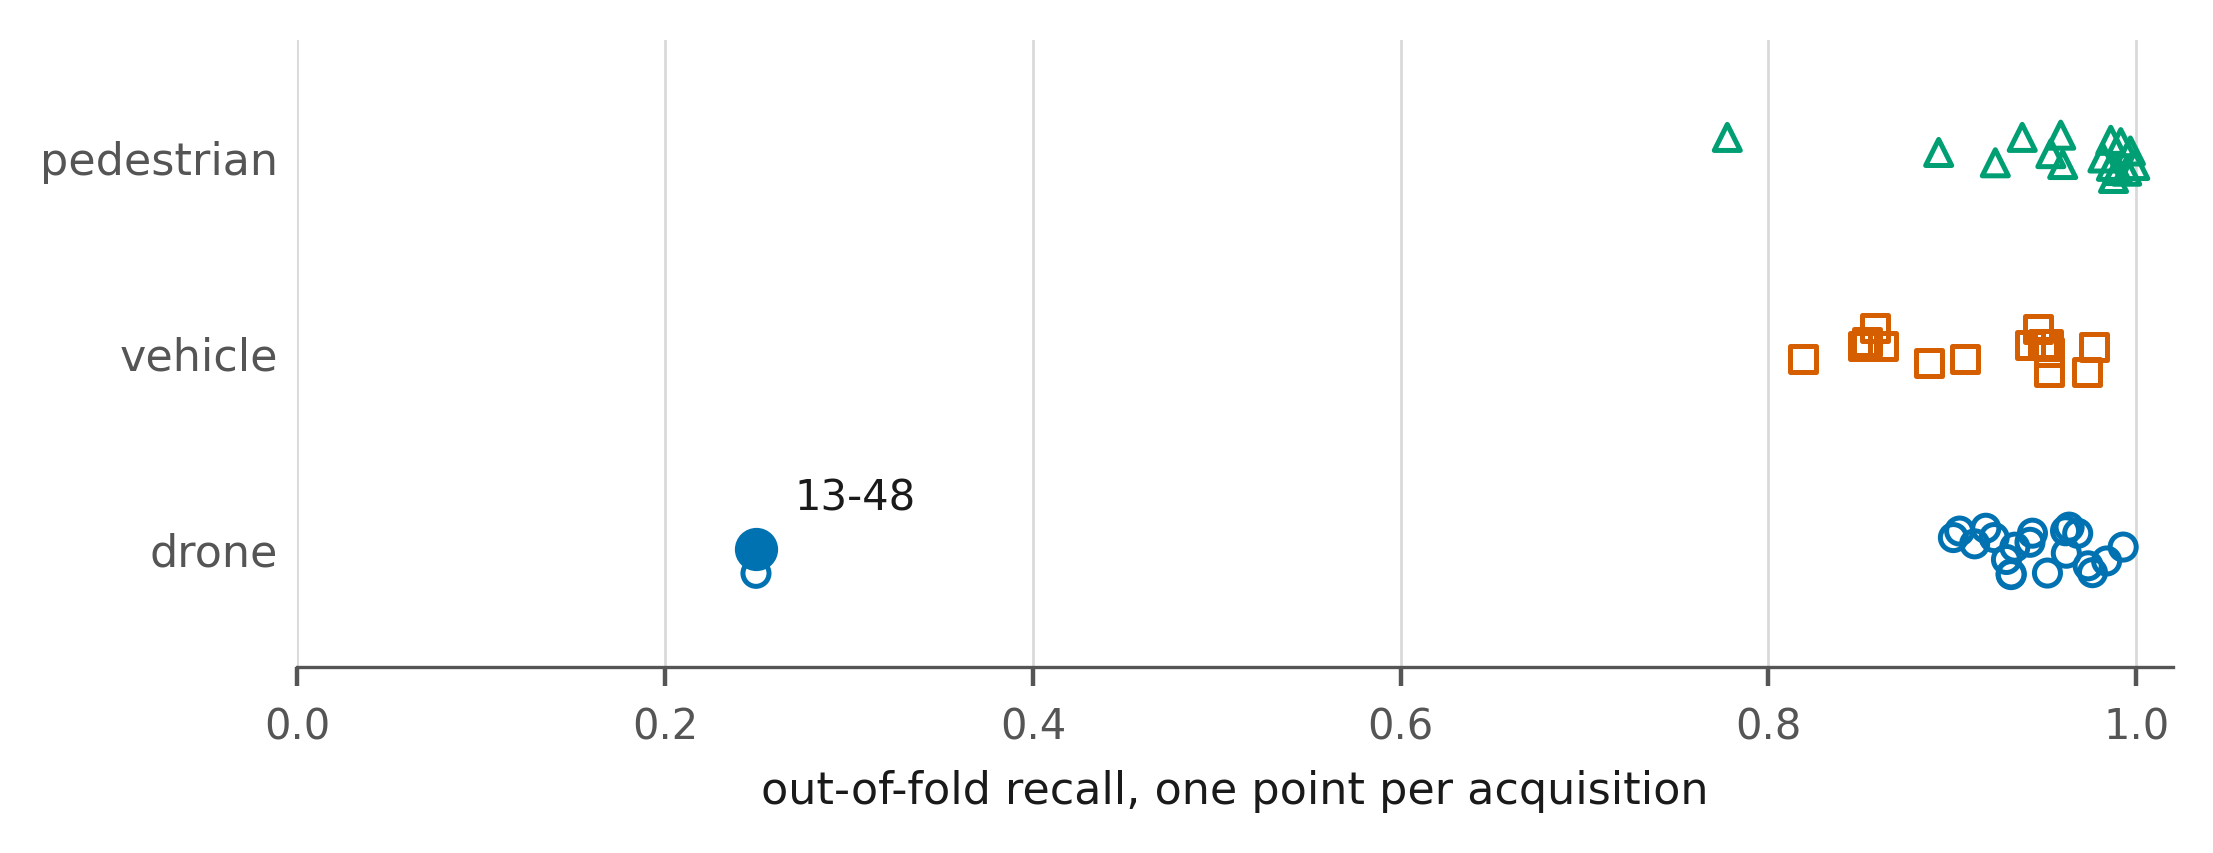
\includegraphics[width=0.74\textwidth]{recall_by_acquisition.png}
\caption{Out-of-fold recall for each of the 52 acquisitions, one point per
unit, vertically jittered within class rows. Forty-three units sit above
0.90 and fifty above 0.78; only \tgt{} falls below 0.75, and it falls to
0.249. The aggregate accuracy of the same cross-validation pass is 0.9099,
which is why the breakdown is the informative view and not a supplement
to it.}
\label{fig:recall}
\end{figure}

Across drone acquisitions, twenty fall above 0.90, between 0.9006 and 0.9929. One, \tgt, is classified at 0.249. The weakest pedestrian and vehicle acquisitions are 0.7776 and 0.8189, so the distribution has a tail in every class, but only one unit in the dataset falls below 0.75 and it falls to a third of that.

Excluding \tgt, the standard deviation of drone recall across acquisitions is 0.0269, \emph{lower} than that of vehicles (0.0522) or pedestrians (0.0567). The drone class therefore does not generalise poorly across acquisitions in general, and a reader who took the aggregate drone recall drop of 0.098 as a statement about drones would draw the wrong conclusion: the apparent class effect, and the outlying fold of Section~\ref{sec:leak}, are both dominated by a single acquisition. With twenty-one drone acquisitions we can show that it dominates the observed distribution; we cannot show that no other acquisition contributes.

\begin{table}[tb]
\caption{Out-of-fold recall for every acquisition, worst first within each
class, from one five-fold grouped cross-validation pass at three seeds. $n$
is the sample count and Hd the median per-sample peak-to-floor headroom in
dB, the quantity Section~\ref{sec:mech} examines. Rounded here only; the
unrounded values and the per-unit seed spread are in the released report.
\tgt{} is bold.}
\label{tab:acq}
\centering
\scriptsize
\setlength{\tabcolsep}{3.4pt}
% GENERATED by tools/make_tables.py. Do not edit by hand.
\begin{tabular}{@{}rrrrrrrrrrrr@{}}
\toprule
\multicolumn{4}{c}{drone} & \multicolumn{4}{c}{vehicle} & \multicolumn{4}{c}{pedestrian} \\
\cmidrule(lr){1-4}\cmidrule(lr){5-8}\cmidrule(lr){9-12}
Acq. & $n$ & Recall & Hd & Acq. & $n$ & Recall & Hd & Acq. & $n$ & Recall & Hd \\
\midrule
\textbf{\texttt{13-48}} & 393 & \textbf{0.2494} & 42.5 & \texttt{15-37} & 370 & 0.8189 & 34.3 & \texttt{11-23} & 308 & 0.7776 & 33.2 \\
\texttt{15-21} & 181 & 0.9006 & 25.8 & \texttt{15-48} & 346 & 0.8512 & 33.8 & \texttt{11-17} & 349 & 0.8926 & 41.7 \\
\texttt{15-33} & 177 & 0.9040 & 27.3 & \texttt{13-44} & 400 & 0.8538 & 36.5 & \texttt{16-00} & 274 & 0.9234 & 44.0 \\
\texttt{12-34} & 660 & 0.9121 & 23.7 & \texttt{13-38} & 317 & 0.8580 & 34.5 & \texttt{16-06} & 258 & 0.9380 & 44.1 \\
\texttt{15-36} & 165 & 0.9182 & 21.7 & \texttt{16-01} & 389 & 0.8625 & 35.0 & \texttt{11-09} & 366 & 0.9536 & 41.0 \\
\texttt{16-09} & 220 & 0.9227 & 28.6 & \texttt{17-09} & 280 & 0.8875 & 40.6 & \texttt{12-57} & 560 & 0.9589 & 36.2 \\
\texttt{15-44} & 170 & 0.9294 & 32.4 & \texttt{13-13} & 581 & 0.9071 & 35.7 & \texttt{15-58} & 200 & 0.9600 & 38.9 \\
\texttt{15-24} & 169 & 0.9320 & 26.8 & \texttt{13-29} & 321 & 0.9424 & 30.7 & \texttt{10-45} & 276 & 0.9819 & 32.7 \\
\texttt{12-41} & 500 & 0.9320 & 18.6 & \texttt{15-42} & 347 & 0.9467 & 34.6 & \texttt{12-29} & 469 & 0.9861 & 47.4 \\
\texttt{15-30} & 212 & 0.9340 & 30.5 & \texttt{16-07} & 434 & 0.9493 & 34.8 & \texttt{12-50} & 703 & 0.9865 & 41.3 \\
\texttt{13-14} & 372 & 0.9422 & 16.9 & \texttt{15-55} & 501 & 0.9521 & 35.2 & \texttt{12-21} & 526 & 0.9876 & 46.3 \\
\texttt{15-42} & 186 & 0.9435 & 26.1 & \texttt{13-19} & 116 & 0.9526 & 39.1 & \texttt{10-53} & 398 & 0.9899 & 50.9 \\
\texttt{15-38} & 176 & 0.9517 & 27.7 & \texttt{13-23} & 625 & 0.9528 & 36.3 & \texttt{11-00} & 297 & 0.9916 & 47.8 \\
\texttt{15-47} & 195 & 0.9615 & 29.8 & \texttt{13-54} & 56 & 0.9732 & 28.9 & \texttt{12-38} & 481 & 0.9948 & 45.4 \\
\texttt{16-11} & 184 & 0.9620 & 32.8 & \texttt{13-49} & 637 & 0.9772 & 34.2 & \texttt{12-43} & 628 & 0.9968 & 46.3 \\
\texttt{16-17} & 178 & 0.9635 & 26.0 &  & & &  & \texttt{12-14} & 607 & 0.9992 & 42.7 \\
\texttt{13-21} & 471 & 0.9682 & 21.2 &  & & &  &  & & &  \\
\texttt{15-50} & 172 & 0.9738 & 29.4 &  & & &  &  & & &  \\
\texttt{15-18} & 42 & 0.9762 & 17.2 &  & & &  &  & & &  \\
\texttt{15-16} & 31 & 0.9839 & 17.0 &  & & &  &  & & &  \\
\texttt{16-15} & 211 & 0.9929 & 25.9 &  & & &  &  & & &  \\
\bottomrule
\end{tabular}

\end{table}

\subsection{What distinguishes it}
\label{sec:distinguish}

We profiled twelve per-sample properties and computed, for each, the standardised difference
\begin{equation}
d \;=\; \frac{\bar{x}_{\tgt} - \bar{x}_{\mathrm{others}}}{s_{\mathrm{others}}},
\label{eq:d}
\end{equation}
the gap in units of the spread among the other twenty drone acquisitions. It is a descriptive effect size, not a test statistic, and we attach no $p$ value to it: with one acquisition on one side there is no sampling distribution to appeal to.

Only five of the twelve properties exceed $|d| = 2$, and two dominate. Doppler centroid sits at bin 8.50 against 30.04 ($d = -15.67$), and peak Doppler bin at 7.58 against 30.01 ($d = -8.16$). The remaining three, headroom, peak level and dynamic range, fall between $+2.07$ and $+2.57$. Range position, range spread and energy extent are unremarkable, with $|d|$ below 0.8. The separation is almost entirely in Doppler position, and no other property comes within a factor of six of it.

\begin{figure}[tb]
\centering
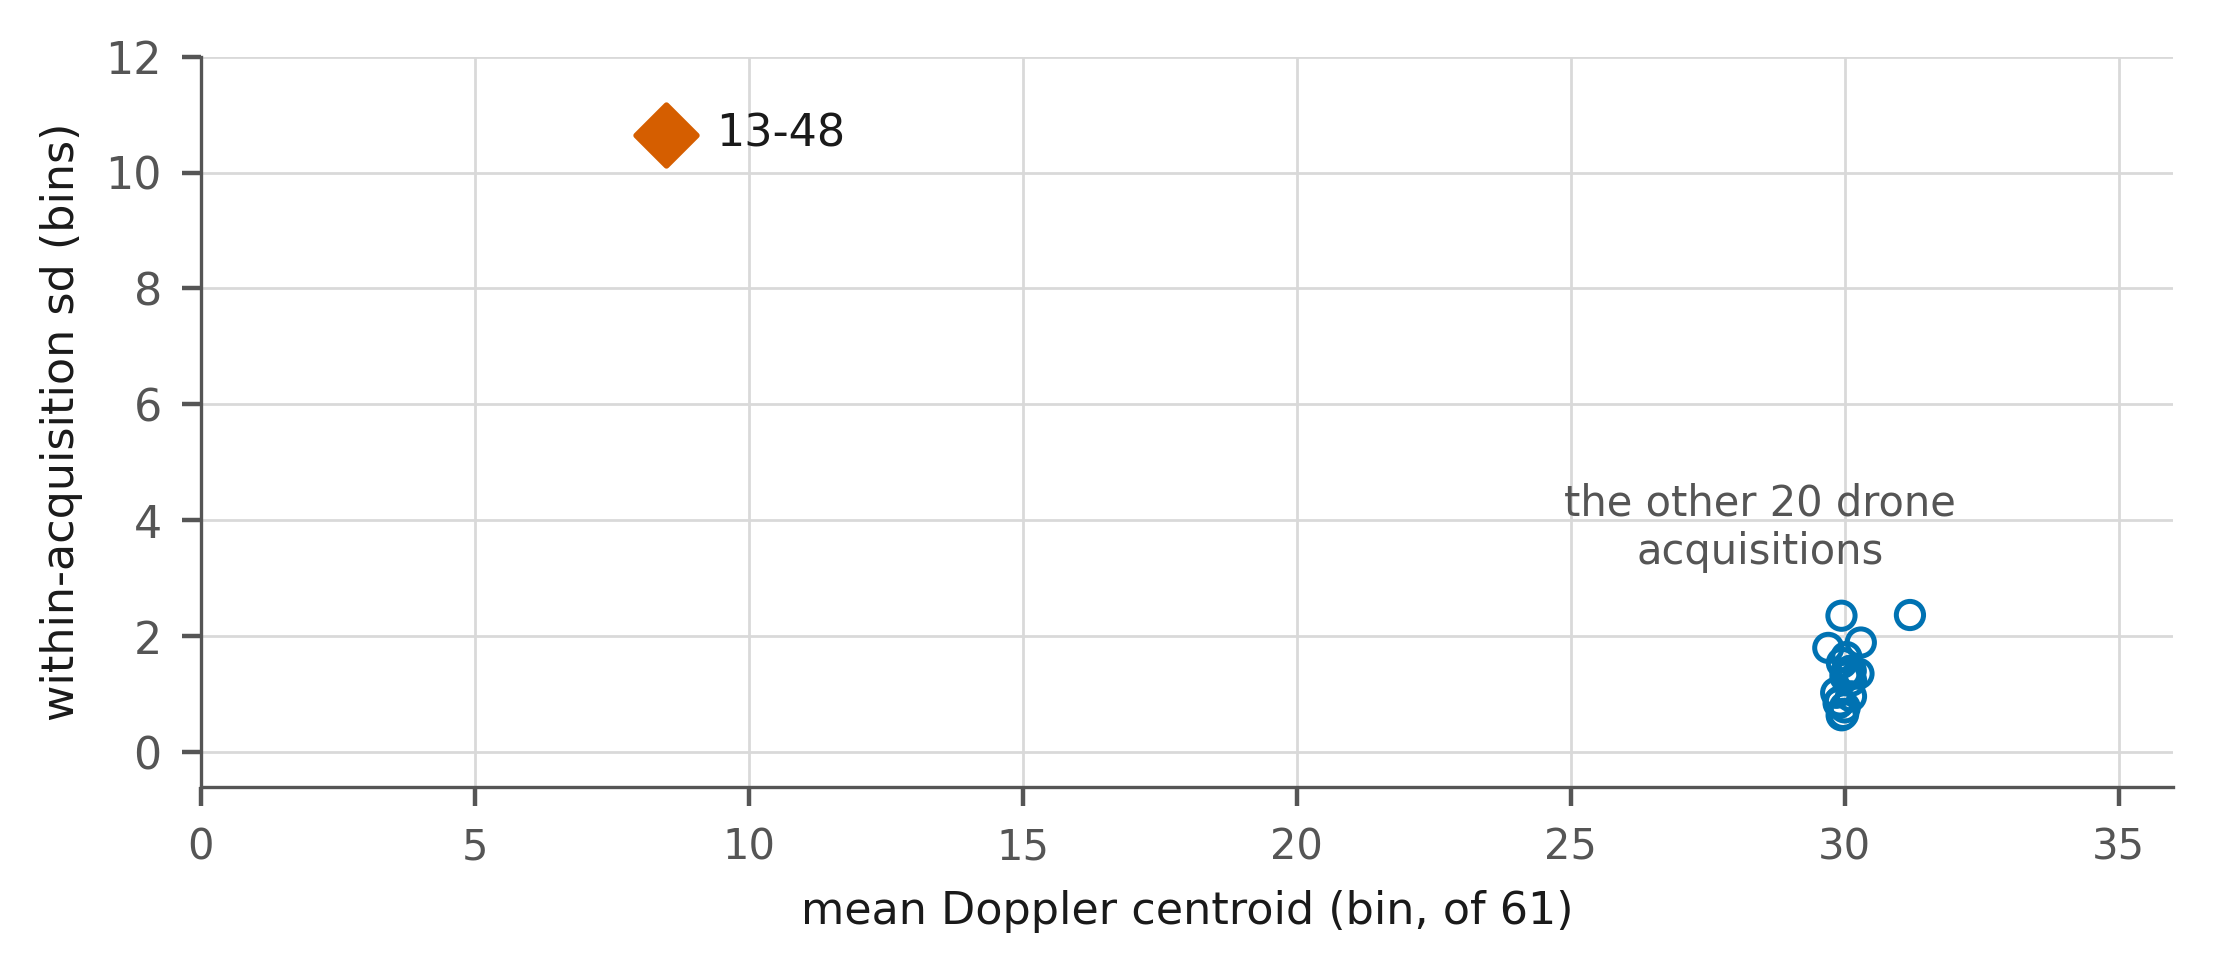
\includegraphics[width=0.6\textwidth]{doppler_by_acquisition.png}
\caption{The 21 drone acquisitions by Doppler centroid and by the spread of
that centroid within the acquisition. Twenty cluster between 29.70 and 31.19
with spreads of 0.64 to 2.37 bins. \tgt{} sits at 8.50 with a spread of
10.64, four and a half times the largest any other shows. It is separated on
both axes at once, so no single threshold on either would be the natural
description of it.}
\label{fig:doppler}
\end{figure}

Figure~\ref{fig:doppler} gives the two-dimensional version of that statement, which is the more informative one. Every other drone acquisition places its target energy at Doppler centroid between 29.70 and 31.19, at the centre of the 61-bin axis, and holds it there, the within-acquisition standard deviation ranging from 0.64 to 2.37 bins. Acquisition \tgt{} places it at 8.50 and does not hold it there, with a standard deviation of 10.64 bins. It is separated from the other twenty both on where its target energy sits and on how much that position varies, and the second of those turns out to matter in Section~\ref{sec:temporal}.

Against class centroids computed from the other acquisitions, 100\,\% of its samples sit nearest the drone centroid. That is consistent with the label rather than evidence for it, and it does not exclude a processing error: a systematic Doppler offset applied to a correctly labelled drone recording would produce exactly this pattern.

\begin{figure}[tb]
\centering
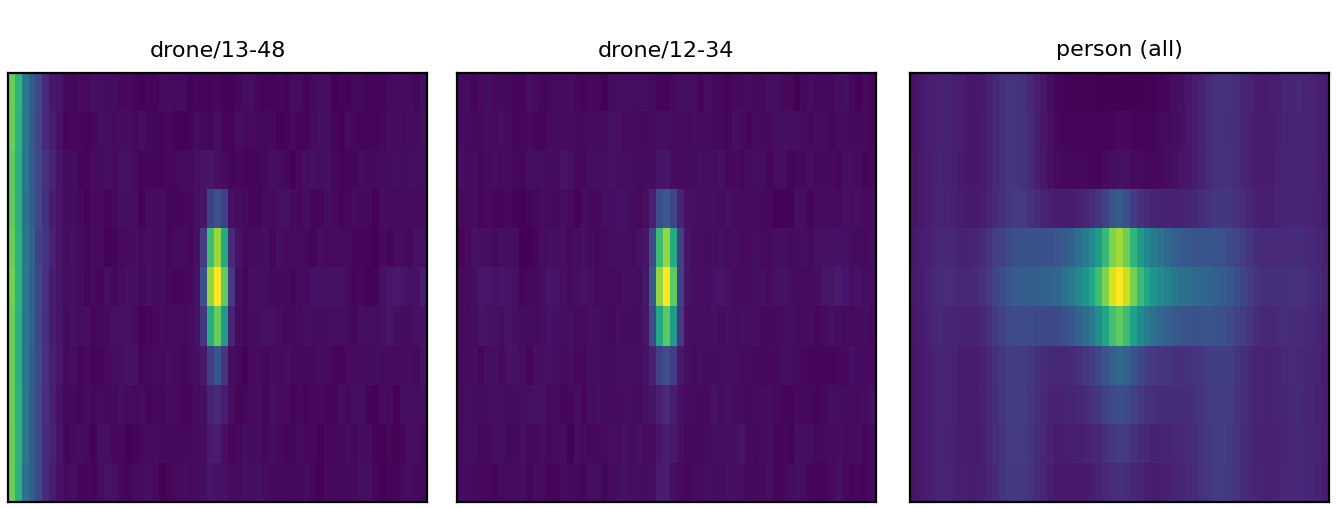
\includegraphics[width=0.66\textwidth]{session_13-48_compact.png}
\caption{Acquisition means, range vertical and Doppler horizontal. \tgt{}
carries a band of energy at the low-Doppler edge that no typical drone
acquisition shows; the pedestrian mean spreads along the Doppler axis, and
79\,\% of held-out \tgt{} is assigned to that class.}
\label{fig:sessions}
\end{figure}

The source publication describes three drone exercises: radial trajectories on autopilot out to 3.1\,km, a circular trajectory at 800\,m, and a free flight with speed and altitude varied manually~\cite{roldan2020,quevedo2019}. Manual free flight can produce more variation in radial velocity than an autopilot trajectory, making the observed Doppler spread consistent with that exercise, though the actual distribution depends on trajectory, orientation and radar geometry, none of which the release records. Acquisition \tgt{} is the only one whose Doppler scatter is an order of magnitude above the rest, so we consider it the likeliest candidate. We stop there rather than asserting it: the publication gives no timestamps linking a folder to an exercise, and a per-recording processing difference cannot be excluded, since an axis convention, a centring change or a crop offset applied to one recording would move energy to an edge just as a genuine velocity distribution would.

\subsection{Coverage test}
\label{sec:coverage}

To separate absence of comparable training data from intrinsic difficulty, we split \tgt{} in half by sample. In the first condition the acquisition is excluded from training entirely and the model is evaluated on one half; in the second, the \emph{other} half is added to the training set and the model is evaluated on the same held-back half. Nothing else changes: same seeds, same architecture, same remaining training pool, and in particular the same test samples, so the conditions are paired sample for sample and the difference between them is attributable to the presence of comparable training data and to nothing else.

\begin{table}[tb]
\caption{Coverage test, mean of ten seeds. Each acquisition is first excluded
from training entirely, then half of it is added back; both conditions are
evaluated on the same held-back half. The two controls were selected after
observing per-acquisition recall and are therefore exploratory rather than
confirmatory.}
\label{tab:coverage}
\centering
\small
\begin{tabular}{@{}llrrrr@{}}
\toprule
Acquisition & Class & $N_{\mathrm{test}}$ & Held out & Half in training & Recovery \\
\midrule
\tgt{}   & drone      & 197 & 0.178 & \textbf{0.948} & \textbf{$+0.770$} \\
\s{11-23} & pedestrian & 154 & 0.800 & 0.856          & $+0.056$ \\
\s{15-37} & vehicle    & 185 & 0.837 & 0.845          & $+0.008$ \\
\bottomrule
\end{tabular}
\end{table}

Recall on the held-back half rises from 0.178 to 0.948 over ten seeds, a recovery of 0.770 (Table~\ref{tab:coverage}). Held out, 79\,\% of samples are assigned to the pedestrian class; with half the acquisition in training, 3\,\% are. The error is therefore not diffuse confusion but a specific and almost complete misassignment, and it is repaired by exposure.

Held-out recall ranges from 0.142 to 0.264 across the ten seeds and the half-in-training condition from 0.904 to 0.980, so the worst seed of one condition still exceeds the best of the other by 0.640. We lead with that separation rather than with a significance test because it assumes nothing about either distribution and is an order of magnitude larger than the spread within either.

The failure is therefore associated with the absence of comparable training examples rather than with an irreducible inability to classify such samples. We stop short of a stronger causal statement, and the limit is structural: because the added samples come from the same acquisition, the experiment cannot separate an out-of-distribution flight regime from an acquisition-specific signature or a per-recording processing difference. What it establishes is that something present in this acquisition and absent from the other twenty is learnable and sufficient.

\subsection{Control acquisitions}
\label{sec:controls}

A large recovery is only evidence of a coverage failure if a large recovery is unusual, and acquisitions well below the aggregate exist in the other classes: the weakest pedestrian and vehicle units sit at 0.7776 and 0.8189. We therefore repeated the identical experiment at the same ten seeds on each. Both were selected after observing per-acquisition recall, so they test whether a large recovery accompanies low recall in the cases available rather than serving as independent confirmatory controls; we return to that limitation in Section~\ref{sec:limits}.

\s{11-23} ($N = 154$) recovers 0.056 and \s{15-37} ($N = 185$) recovers 0.008, the latter indistinguishable from zero: its conditions overlap on nine of ten seeds with a per-seed standard deviation of 0.030. All three acquisitions sit well below their class aggregate, yet exposure repairs one and leaves the other two where they were. Low recall and a large recovery are therefore separate properties, and the coverage result is not a restatement of \tgt{} being difficult.

The controls also differ descriptively, which makes the contrast interpretable rather than merely numerical. \s{11-23} is unremarkable in Doppler but an outlier in energy extent ($d = +3.4$) with 56.8\,\% of its frames nearest the \emph{drone} centroid: confusable with another class rather than unrepresented, which training data should not repair. \s{15-37} is the cleaner control. No property separates it from other vehicle acquisitions, the largest standardised difference across the twelve being 0.25 against $-15.67$ for \tgt, and 62.7\,\% of its frames sit nearest their own class. It is an ordinary acquisition simply handled less well. An acquisition can therefore be weak without being unrepresented, which is precisely the alternative the coverage experiment has to exclude.

This is the paper's principal result, and it concerns this benchmark: a classifier whose aggregate score looks healthy fails severely on one of the dataset's acquisitions, and the standard evaluation gives no indication of it. The rest of the paper asks whether any change to the input or the model repairs it.

% =====================================================================
\section{Approximate Temporal Context}
\label{sec:temporal}

The strongest objection to the above is that our model sees one frame while the published baseline sees three, so the failure might be an artefact of our input rather than a property of the benchmark. This section addresses that by measurement. The experiments use our own compact network with an approximate three-frame input; they do not reproduce DopplerNet and cannot determine how DopplerNet would perform on \tgt.

\subsection{What the published numbers measure}
\label{sec:published}

Our classifier reaches 0.9335 under grouped five-fold cross-validation and 0.9537 on a single random partition, against the 99.48\,\% reported for DopplerNet and the 98.08\,\% for the lighter reference. Before attributing that gap to anything we state what the three numbers measure, because they do not measure the same thing and the differences run in opposite directions.

DopplerNet's figure is a five-fold cross-validated mean, obtained by splitting the data at random into five subsets and averaging the five resulting confusion matrices~\cite{roldan2020}. That is the same protocol as our 0.9335, so the comparison is like for like and the gap is 6.1 points, none of which protocol explains. Two documented differences remain: DopplerNet has 3\,818\,755 parameters against our 101\,139, a factor of thirty-eight, and its input is an $11 \times 61 \times 3$ distance-Doppler-time tensor, three time-consecutive detections stacked as channels and separated by 400\,ms, a choice the source publication justifies through the classification latency each added frame costs.

The lighter reference differs in the other direction. Its 0.9808 is reported as a peak validation accuracy on an 80/20 split with no separate test set~\cite{zhang2025}: the best epoch's accuracy, measured on the same data used to choose that epoch. Our 0.9537 is test accuracy on data withheld from both training and model selection, and the reference architecture is within three hundred parameters of ours on the same single-frame input. We draw no conclusion from the size of that particular difference, only that the two quantities are not comparable, and we report ours at the more conservative of the two definitions.

Nor can a user of the release remove the input difference. The archive supplies one CFAR-cropped matrix per detection with no timestamp and no frame counter, the only ordering information being the trailing integer in each file name, so the 400\,ms triplets are not reconstructible from the public data by anyone and a headline accuracy obtained from an input the release does not retain cannot be reproduced from it. We treat that as part of the paper's subject rather than an aside: it is a reporting problem of the same family as the one studied here, in which the published number is correct for what it measures and the release does not carry what a reader needs in order to see what that is.

\subsection{Four arms}

We can nevertheless approximate the formulation and measure whether the approximation carries temporal information rather than assuming it. Triplets form within each folder from consecutive file-name integers, never across a gap, giving 17\,221 triplets from 17\,485 frames and 391 on \tgt. Four arms are compared at ten shared seeds on the same triplet centres, so the comparison is paired sample for sample: \emph{single}, the centre frame alone, replicated to three channels so channel count is held fixed; \emph{index}, the two index-adjacent neighbours, the closest available approximation to the published construction; \emph{clean}, the nearest neighbours carrying the centre's own split tag, so no window crosses the partition, at mean companion distance 2.57; and \emph{shuffle}, two frames drawn at random from the same folder, never the true neighbours, which is a transductive same-acquisition context rather than a deployable one. All three multi-frame arms hold channel count, folder, labels and sample count fixed, so the ordering assumption and the window overlap both become testable rather than assumed, and three channels take the model from 101\,139 to 102\,291 parameters, so capacity is not what separates them.

\begin{table}[tb]
\caption{Approximate three-frame context, ten seeds; random-split figures are
three seeds. $d$ is the mean index distance of the companion frames from the
centre. \tgt{} recall is under the held-out protocol, the acquisition being
absent from training entirely. This is our own network, not DopplerNet.}
\label{tab:temporal}
\centering
\small
\begin{tabular}{@{}llcrr@{}}
\toprule
Arm & Companions & $d$ & Random split & \tgt{} recall \\
\midrule
single  & none            & --   & 0.9516 $\pm$ 0.0046 & 0.2379 $\pm$ 0.0428 \\
index   & adjacent        & 1.00 & 0.9794 $\pm$ 0.0016 & 0.3673 $\pm$ 0.0661 \\
clean   & same split tag  & 2.57 & 0.9731 $\pm$ 0.0080 & 0.4634 $\pm$ 0.0970 \\
shuffle & folder-wide     & --   & 0.9932 $\pm$ 0.0016 & 0.5435 $\pm$ 0.1257 \\
\bottomrule
\end{tabular}
\end{table}

\subsection{Temporal context raises aggregate accuracy and does not fix the acquisition}

A three-frame input raises random-split accuracy from 0.9516 to 0.9794, within a quarter of a point of the 0.9808 reported for the lighter published model. The approximation therefore reaches the published operating point for a model of this size, which is what makes the second half of the result meaningful.

That same classifier still fails on \tgt. Recall under the held-out protocol rises from 0.238 to 0.367, a paired gain of $+0.129$ over ten seeds ($t = +4.82$), so the gain is real and the majority of the acquisition's frames are still assigned to the wrong class. \textbf{The failure is therefore not an artefact of the single-frame input, and it persists while aggregate accuracy rises by 2.8 points.} Even the shuffle arm at 0.9932 leaves \tgt{} at 0.544, far below both the 0.90 or better of other acquisitions and the 0.948 obtainable once the acquisition is represented in training at all. Every configuration we tested fails on it, and the one intervention that does not fail is exposure.

\subsection{What the window overlap is worth}

The second result we did not anticipate, and it corrects what the audit alone would have suggested. A sliding window over a frame-level random split does put test frames inside training inputs on a large scale: 50.6\,\% of training triplets hold at least one test frame, and 82.7\,\% of all test frames appear inside some training input under index order, against 68.4\,\% under shuffled companions, each within a point of what the partition's proportions predict.

On that evidence one would expect the three-frame gain to be substantially leakage. The \emph{clean} arm measures what it is actually worth, and the audit reports exactly zero overlap for it. Removing the overlap costs 0.0063 in accuracy, 0.9794 against 0.9731, which at three seeds is inside the spread of either arm. So although four fifths of the test set appears somewhere in training, the inflation from it is well under a point for this model and this window construction, and three frames still beat one by 0.0215 with no overlap at all. A longer context, a different stride or a larger model could weigh it differently, so we make no general claim about sliding windows, and we report this in both directions because the audit alone would have supported a stronger claim than the experiment does.

\subsection{Companion distance is what separates the arms}

What does separate the arms is how far the companions sit from the centre. Recall on \tgt{} rises monotonically with that distance: 0.367 for index-adjacent frames at $d = 1$, 0.463 for the nearest same-tag frames at $d = 2.57$, and 0.544 for companions drawn from anywhere in the folder. Adjacent detections are nearly redundant, 400\,ms apart in a continuous recording, while more distant ones sample the acquisition's internal variability. That variability is largest precisely here, the Doppler centroid of \tgt{} having a standard deviation of 10.64 bins against 0.64 to 2.37 elsewhere, so a distant companion carries more new information in this acquisition than it would in any other.

The shuffle arm is also transductive, drawing on other test frames at inference time as a system classifying a live stream could not, so \emph{index} is the deployment-realistic arm and 0.367 is the figure the comparison rests on. That the arms are not exchangeable is itself informative about the release: had file-name order been arbitrary, index and shuffle would have differed only by chance rather than by 0.176 ($t = -4.35$ over ten paired seeds). The trailing integer therefore does track acquisition order closely enough to matter, which is worth recording for anyone else working with this archive, since the release does not document it.

% =====================================================================
\section{Input Resolution and Numerical Precision}
\label{sec:compress}

Deployed radar classifiers run under memory and bandwidth constraints, and the established finding in vision is that compression damages some parts of the input distribution more than the aggregate reveals~\cite{hooker2019,hooker2020,tran2022}. That is the same shape of claim as this paper's, so it is worth testing on the same data. The result is mostly negative.

\subsection{Method}

Two axes are varied independently. \emph{Input aggregation} averages adjacent Doppler bins by a factor of 1, 2, 4 or 8, reducing the $11 \times 61$ crop to as few as 11 columns by 8. \emph{Weight precision} quantises to 32, 16, 8 or 4 bits. The sixteen combinations are each evaluated on the standard grouped split and, separately, with \tgt{} held out of training entirely, so the grid is scored both on the distribution it was trained on and on the acquisition that was already failing. Three seeds per cell for the grid, ten for the subset in Section~\ref{sec:compress-ten}. Because normalisation is a fixed affine map, quantising before or after it is equivalent up to a scale factor, so the bit-width axis is not confounded with the normalisation choice.

\subsection{The standard split is flat; the held-out acquisition is not}

\begin{table}[tb]
\caption{Input aggregation by weight precision, three seeds per cell.
Standard split columns are grouped-protocol accuracy and drone recall.
Held-out columns are recall on \tgt{} with the acquisition absent from
training, which is why they are an order of magnitude lower and far noisier:
that column is a single acquisition at three seeds, not an aggregate.}
\label{tab:compress}
\centering
\small
% GENERATED by tools/make_tables.py. Do not edit by hand.
\begin{tabular}{@{}lrrrrr@{}}
\toprule
& & \multicolumn{2}{c}{Standard split} & \multicolumn{2}{c}{Held-out \texttt{13-48}} \\
\cmidrule(lr){3-4}\cmidrule(lr){5-6}
Aggregation & Bits & Accuracy & Drone recall & Recall & sd \\
\midrule
$1\times$ & 32 & 0.9357 & 0.8952 & 0.1934 & 0.0331 \\
 & 16 & 0.9433 & 0.9199 & 0.2061 & 0.0382 \\
 & 8 & 0.9390 & 0.8932 & 0.2023 & 0.0344 \\
 & 4 & 0.8229 & 0.6523 & 0.1870 & 0.0089 \\
\addlinespace[2pt]
$2\times$ & 32 & 0.9479 & 0.9154 & 0.3562 & 0.0789 \\
 & 16 & 0.9442 & 0.9041 & 0.2519 & 0.0891 \\
 & 8 & 0.9449 & 0.9080 & 0.4415 & 0.2074 \\
 & 4 & 0.9068 & 0.8417 & 0.0636 & 0.0636 \\
\addlinespace[2pt]
$4\times$ & 32 & 0.9461 & 0.9288 & 0.4898 & 0.1056 \\
 & 16 & 0.9475 & 0.9209 & 0.5776 & 0.0687 \\
 & 8 & 0.9388 & 0.9045 & 0.5127 & 0.1107 \\
 & 4 & 0.7504 & 0.4120 & 0.1858 & 0.0814 \\
\addlinespace[2pt]
$8\times$ & 32 & 0.9185 & 0.8506 & 0.1934 & 0.0127 \\
 & 16 & 0.9192 & 0.8477 & 0.1794 & 0.0089 \\
 & 8 & 0.9275 & 0.8922 & 0.2061 & 0.0305 \\
 & 4 & 0.9046 & 0.8348 & 0.1501 & 0.0153 \\
\bottomrule
\end{tabular}

\end{table}

On the standard split, accuracy sits between 0.9185 and 0.9479 in twelve of the sixteen cells (Table~\ref{tab:compress}), and the four exceptions are exactly the 4-bit column: 0.8229, 0.9068, 0.7504 and 0.9046 at $1\times$ to $8\times$. Precision is therefore the only axis that damages the aggregate, and only at its most extreme setting. Fourfold Doppler aggregation at 16 bits, which discards three quarters of the input columns and half the weight precision, scores 0.9475 against 0.9357 at full resolution and full precision. The standard split is, to the resolution this experiment can see, indifferent to compression until precision collapses.

The held-out column behaves differently, and in a direction we did not predict. Recall on \tgt{} rises from 0.1934 at $1\times$ to 0.4898 at $4\times$ in 32-bit, and from 0.2023 to 0.5127 in 8-bit. Aggregating the Doppler axis, which destroys information, \emph{helps} on the acquisition whose distinguishing property is Doppler position. That is interpretable: coarsening the axis along which the acquisition is displaced makes the displacement smaller in units of the representation. At $8\times$ the effect reverses completely, back to 0.1934 and 0.2061, so there is an optimum rather than a monotone trend, $8\times$ leaving only eight Doppler columns.

\subsection{A ten-seed subset, and how noisy the held-out column is}
\label{sec:compress-ten}

Three seeds on a single acquisition is not enough to rest anything on, and the standard deviations in Table~\ref{tab:compress} make that visible: the $2\times$ 8-bit cell reports 0.4415 with a standard deviation of 0.2074. We therefore reran eight cells at ten seeds. The gap between the standard split and the held-out acquisition is 0.6988 at $1\times$ 32-bit, 0.6027 at $2\times$, 0.5082 at $4\times$ and 0.7095 at $8\times$, with the 8-bit row tracking closely at 0.6894, 0.6082, 0.5268 and 0.7217, so the ordering of the four aggregation factors holds under both seed counts and both precisions. That ordering is the part of the grid result we consider stable. At ten seeds and 32 bits, held-out recall on \tgt{} is 0.2221 at $1\times$ against 0.3975 at $4\times$, a mean per-seed gain of 0.175 that is positive on ten of ten seeds with a paired $t$ of $+4.24$. That is the figure we quote for the effect, and the standard split over the same ten seeds shows no corresponding change, a paired $t$ of 1.05.

\subsection{It does not generalise across acquisitions}

If fourfold aggregation were a method rather than a coincidence it would help other acquisitions too, so we held out each of five in turn at three seeds, at $1\times$ and $4\times$: the three largest drone units including \tgt, plus the two controls of Section~\ref{sec:controls}. The per-acquisition changes are $+0.136$ for \tgt, $+0.048$ for \s{15-37}, $+0.020$ for \s{15-21}, $-0.017$ for \s{12-34} and $-0.022$ for \s{11-23}. Three of the five improve and two worsen, the mean change is $+0.033$ with a paired $t$ of 1.16 on four degrees of freedom, and an exact sign test gives $p = 0.50$ one-sided. Nothing here survives being asked whether it generalises, and the effect on \tgt{} is roughly three times the next largest.

We therefore present fourfold aggregation as something that helps this acquisition, for a reason specific to how it differs, and not as a recommendation. Reporting it as a technique on the strength of the $+0.136$ alone would be exactly the error this paper is about.

\subsection{Resolution and precision interact weakly, or not detectably}

To ask whether the two axes interact rather than simply add, we formed the factorial contrast
\begin{equation}
I \;=\; Y_{\mathrm{both}} - Y_{\mathrm{input}} - Y_{\mathrm{weights}} + Y_{\mathrm{neither}}
\label{eq:interaction}
\end{equation}
within each seed, comparing aggressive aggregation and aggressive quantisation applied separately and together. Per-seed values are $-0.2595$, $+0.2973$, $-0.0476$, $-0.1393$ and $+0.0366$, giving a mean of $-0.0225$, a bootstrap 95\,\% confidence interval over seeds of $[-0.1748, +0.1410]$ and $t = -0.24$ on four degrees of freedom. The interval includes zero and is wide. The honest summary is that this experiment is inconclusive about interaction, not that the axes are additive: a moderate interaction would not have been detected at five seeds with this spread. We state it that way because the opposite framing, that compression axes combine additively, is the kind of claim that propagates.

Across the grid, the standard split loses less than two points to any configuration keeping 8 or more bits, and the clearest effect on the failing acquisition is positive over much of the range. We did not find the disparate-impact pattern that compression research in vision reports, on this dataset, with this architecture and these two axes. That is one non-replication on one benchmark; it does not weigh against the vision results, and the likeliest explanation is the simplest, that an $11 \times 61$ CFAR crop carries far less redundant structure to lose than a natural image.

% =====================================================================
\section{Mechanisms Considered and Not Supported}
\label{sec:mech}

Four physically motivated mechanisms for the drone class being more fragile were formulated before the measurements, and none was supported by the measurements we could make. We report them because a reader will think of them, and because which ones the data cannot reach is itself informative about the release.

\textbf{Rotor sideband loss.} Blade returns produce sidebands at Doppler offsets the supplied crops do not span, the retained window being approximately 21\,km/h. This mechanism is not testable on this release at all, and we say so rather than reporting a null result that would be an artefact of the crop.

\textbf{Low redundancy from compact energy.} Drone returns occupy fewer cells than a vehicle's, so there is less redundant structure to survive a perturbation. The compression grid of Section~\ref{sec:compress} is the test and does not support the mechanism: drone recall on the standard split tracks overall accuracy closely across the grid rather than degrading faster.

\textbf{Limited dynamic-range headroom.} Across drone acquisitions, median peak-to-floor headroom correlates with out-of-fold recall at Pearson $-0.62$, which looks like a mechanism. It is not one. Removing \tgt{} alone takes the correlation to $-0.16$. The apparent relationship is one point, and \tgt{} has the largest headroom of any drone acquisition at 42.5\,dB against a class median near 26 (Table~\ref{tab:acq}), so the correlation reflects that one unit being extreme on both axes rather than headroom predicting recall.

\textbf{Doppler positional insensitivity.} If the network were insensitive to where energy sits on the Doppler axis a displaced acquisition would not be a problem; if it were too sensitive, shift augmentation should fix it. We tested the second: random Doppler shifts of $\pm 4$, $\pm 8$ and $\pm 16$ bins during training give held-out recall on \tgt{} of 0.1608, 0.1613 and 0.1603, against 0.2214 without augmentation. Every strength makes it worse, and none approaches the 0.4641 that fourfold aggregation reaches on the same protocol, so simply teaching the model that Doppler position may vary is not what this acquisition needs.

Each of these is a measurement that failed to support an explanation rather than one that excludes the physics, which in several cases our data cannot reach. We draw one conclusion from the set: the coverage experiment of Section~\ref{sec:coverage}, which manipulates exposure and changes recall by 0.770, is the only intervention among everything we tried that moves this acquisition substantially, and the mechanism it implicates is the composition of the training set rather than any property of the signal.

% =====================================================================
\section{Discussion and Limitations}
\label{sec:discussion}

\subsection{What the results do and do not support}

The coverage result is the finding we consider established: a measured effect of 0.77 in recall with no overlap between conditions on any of ten seeds, a controlled manipulation isolating within-acquisition coverage, two controls on which the same manipulation does nothing, and a descriptive signature identifying the acquisition without reference to classifier performance at all. What it does not identify is which physical or processing factor makes that coverage necessary, for the reason given in Section~\ref{sec:coverage}: the added samples come from the same acquisition as the test samples, so flight regime, acquisition signature and processing difference move together.

The recommendation follows, with its scope stated. For datasets assembled from continuous acquisitions, where deployment requires generalising to recordings absent from training, aggregate accuracy should be accompanied by an acquisition-level breakdown, which costs nothing: every unit is held out exactly once in a grouped cross-validation, so the breakdown is a by-product of a pass already being run. Where deployment operates on the benchmark's own distribution, frame-level evaluation may be appropriate and we make no claim against it.

What the acquisition represents we cannot settle, and the two readings have different consequences. A low-Doppler band could follow from flight dynamics, in which case a deployment consequence follows directly: a classifier trained on this benchmark would fail on a flight regime it had not seen. It could equally follow from a recording-specific processing difference such as an axis convention, a centring change or a crop offset, in which case the finding is about the dataset rather than about radar classification. The release carries no metadata separating them, so we state the evaluation finding, which holds under either reading, and leave the physical one open.

\subsection{Limitations}
\label{sec:limits}

Both principal findings rest on the same acquisition, so the effective sample size at the level of flight regimes is one. The data comes from one dataset, one radar and one drone platform, with \tgt{} comprising 7.8\,\% of the drone samples. Whether the same phenomenon appears under other architectures, or on another radar or benchmark, is untested here.

The two controls show that the large recovery was not observed in either, but three acquisitions of fifty-two is a contrast of three cases rather than a law about difficult recordings, and both controls were chosen after seeing per-acquisition recall. Selecting controls on the dependent variable is a real weakness of the design. The remedy is to stop selecting, and the experiment that would settle it is the same coverage test run on all 52 units, turning the claim from a comparison of three hand-picked cases into a distribution, and allowing the direct test of whether low baseline recall predicts recovery in general. We have not run it, and we name it as the obvious next step rather than leaving the reader to notice the gap.

The aggregation effect of Section~\ref{sec:compress} is likewise specific to \tgt: across five acquisitions tested one at a time it neither generalises nor reaches significance, and we present it as acquisition-specific accordingly. The grouping rule of Section~\ref{sec:grouping} is an inference from directory structure rather than a ground-truth identifier, though as noted there it cannot affect any drone result, since all 21 drone folders map one to one onto units.

Finally, our network is not DopplerNet, and the three-frame arms of Section~\ref{sec:temporal} are an approximation to its input that the release does not permit reconstructing exactly. We cannot say how DopplerNet would perform on \tgt. What we can say is that every configuration we tested, including one matching the best published accuracy for a model of this size, fails on it.

% =====================================================================
\section{Conclusion}
\label{sec:conclusion}

On the Real Doppler RAD-DAR benchmark, grouping by inferred acquisition exposes heterogeneity that aggregate frame-level accuracy does not show, and it is concentrated in one recording. Acquisition \tgt{} fails under every configuration we tested: an approximate three-frame input that reaches 0.9794 random-split accuracy, within a quarter of a point of the best published figure for a model of this size, leaves it at 0.367; sixteen combinations of input resolution and weight precision never take it above 0.578; and Doppler shift augmentation at three strengths makes it worse. The only intervention that repairs it is putting part of the acquisition into training, which takes recall on a held-back half from 0.178 to 0.948 with no overlap between conditions on any of ten seeds, while the weakest acquisition of each other class recovers 0.056 and 0.008. The problem is coverage.

These results establish a benchmark-specific case study rather than a general law. They do support reporting acquisition-level performance wherever a dataset is assembled from continuous recordings, since the breakdown costs one cross-validation pass that was already being run. Code, partition files, per-stage reports and a script that rechecks every number reported here against its own tolerance are released at \url{https://github.com/falcon-colab/rdrd-acquisition-coverage} and archived at~\cite{dataset2026}.

\section*{Reproducibility}

The repository contains the preparation pipeline, the exact partition files, the per-stage JSON reports from which every number in this paper is taken, and \texttt{check\_expected.py}, which re-reads those reports and verifies each reported figure against a stated tolerance with a recorded justification for that tolerance. Tables~\ref{tab:acq} and~\ref{tab:compress} are generated from their reports by \texttt{tools/make\_tables.py} rather than typed, so a transcription error cannot enter them. Running the checker on a fresh clone reproduces the verification without a GPU.

% =====================================================================
{\small
\begin{thebibliography}{99}
\itemsep1pt \parskip0pt \parsep0pt

\bibitem{roldan2020} I.~Roldan, C.~R.~del-Blanco, \'A.~Duque de Quevedo \emph{et al.}, ``DopplerNet: a convolutional neural network for recognising targets in real scenarios using a persistent range--Doppler radar,'' \emph{IET Radar, Sonar \& Navigation}, vol.~14, no.~4, pp.~593--600, 2020.

\bibitem{quevedo2019} \'A.~Duque de Quevedo, F.~Ib\'a\~nez Urzaiz, J.~Gismero Menoyo and A.~Asensio L\'opez, ``Drone detection and radar-cross-section measurements by RAD-DAR,'' \emph{IET Radar, Sonar \& Navigation}, vol.~13, no.~9, pp.~1437--1447, 2019.

\bibitem{zhang2025} L.~Zhang, G.~Tu, Y.~Xu and X.~Zhou, ``A lightweight CNN-based method for micro-Doppler feature-based UAV detection and classification,'' \emph{Electronics}, vol.~14, no.~24, art.~4831, 2025.

\bibitem{buchman2022} D.~Buchman, M.~Drozdov, T.~Krilavi\v{c}ius \emph{et al.}, ``Pedestrian and animal recognition using Doppler radar signature and deep learning,'' \emph{Sensors}, vol.~22, no.~9, art.~3456, 2022.

\bibitem{chen2025} L.~Chen, N.~Zhu, H.~Chen \emph{et al.}, ``A causality-inspired single-source domain generalized method for low-slow-small threat target recognition through holographic Doppler radar,'' \emph{Expert Systems with Applications}, vol.~287, art.~128104, 2025.

\bibitem{bai2026} B.~Bai, L.~Xue, M.~Xue and B.~Pu, ``Open-set recognition of radar one-dimensional range profiles based on attention mechanism and multi-task joint training,'' \emph{IET Radar, Sonar \& Navigation}, vol.~20, no.~1, art.~e70121, 2026.

\bibitem{dietterich1998} T.~G.~Dietterich, ``Approximate statistical tests for comparing supervised classification learning algorithms,'' \emph{Neural Computation}, vol.~10, no.~7, pp.~1895--1923, 1998.

\bibitem{nadeau2003} C.~Nadeau and Y.~Bengio, ``Inference for the generalization error,'' \emph{Machine Learning}, vol.~52, no.~3, pp.~239--281, 2003.

\bibitem{hooker2019} S.~Hooker, A.~Courville, G.~Clark, Y.~Dauphin and A.~Frome, ``What do compressed deep neural networks forget?'' arXiv:1911.05248, 2019.

\bibitem{hooker2020} S.~Hooker, N.~Moorosi, G.~Clark, S.~Bengio and E.~Denton, ``Characterising bias in compressed models,'' arXiv:2010.03058, 2020.

\bibitem{tran2022} C.~Tran, F.~Fioretto, J.-E.~Kim and R.~Naidu, ``Pruning has a disparate impact on model accuracy,'' in \emph{Advances in Neural Information Processing Systems}, vol.~35, 2022, pp.~17652--17664.

\bibitem{dataset2026} G.~Mustafa, ``Code and analysis for this paper,'' Zenodo, 2026, doi:10.5281/zenodo.23118075.

\end{thebibliography}}

\end{document}
